\chapter{Implementation}
\label{cha:implementation}

As mentioned above this project's tool consists of two parts, 
the web application where users create and upload textbooks and questions for their common 
topics and the alexa skill which is the main interaction tool used to study and practice.

\section{Web Application}

The web application is a full stack server that communicates both with the website as well 
as the alexa skill. It is a platform where users can administrate and have an overview of 
all the available topics, questions, textbooks as well as the ones created by the user.

The architecture principles behind the design of this web application are the following:
it aspires to be scalable, extensible, flexible and modern. Why exactly these adjectives
and not others? Well, as any living platform, the application will hopefully change and
develop over time, if it is going to be used. Since one important criterion is to 
create Communities of Practice overtime, by connecting users who intend to study
similar topics, the software will have to be adaptable to any changes that might occur 
in the future and so it needs to be scalable. Users will determine in what direction 
the software should go, what features need to be added to make the whole studying 
process of interacting with the website and uploading questions easier and more useful
overtime, so it needs to be extensible. It needs to be flexible to changes, so it 
adapts in any direction required and it needs to be modern to both take full advantage
of the latest available technologies and ideas as well as pleasant to use, specially
for users in the habit and knowledge of the latest technologies.

The server side of this web application communicates both with the front-end shown
in the browser, but also with the alexa skill, which fetches all the data stored 
in the database.


\section{Programming Environment}

\subsection{Major Technologies}
With the later in consideration, the programming technologies selected needed to regard
exactly those aspects, so the system was developed with the following:


\begin{itemize}
\item \textbf{ReactJS:} Statistically the most widely used front-end framework, React
    was created by the Facebook Team back in 2013. The most characteristic feature 
    of React is its component-center design. In React the developers can very easily
    separate concerns by extracting HTML, CSS and JavaScript from small snippets and
    create "Components" which are higher level Abstractions of reusable pieces of code
    that live in the application in a very Object-Oriented style.

    With React the developers can in a very clean way extend or replace small pieces 
    of their web application making it the perfect choice of technology to develop this
    volatile learning platform, likely to change in any direction as required by its
    users.

\item \textbf{TypeScript:} A superset of JavaScript, TypeScript as the name implies
    creates a layer of security over normal JavaScript code by statically analyzing 
    types at compilation. This makes development safer, as it automatically covers 
    most of the use needed by unity testing and showing the developer most potential dynamic 
    bugs at compile time and making them obvious when refactoring/adapting and 
    extending.


\item \textbf{Go:} The choice for back-end was Google's young Programming Language, Go.
    It provides the same advantages of TypeScript with its strict typing system. 
    It also makes use of concurrency fairly easy, with its plain and simple syntax, making
    it a very performant choice for the server that communicates with the front-end 
    and alexa skill.

\item \textbf{MongoDB:} A NoSQL database architecture, very performant and based on
    JavaScript Object Notation (JSON) syntax, which is also used by all alexa skills to
    communicate via HTML. It 

\item \textbf{Auth0:} \textit{a flexible, drop-in solution to add authentication and 
    authorization services to your applications. Your team and organization can 
    avoid the cost, time, and risk that comes with building your own solution to 
    authenticate and authorize users} \cite{auth0}. It is a perfect extension to add user 
    functionalities to the web application by safeguarding their privacy and data with
    a third party library specialized just in that.

\item \textbf{Gorilla/Mux:} One of the most popular and well written server side 
    frameworks written in the Go Programming Language, Mux aspires to create a perform
    transition between server and single page requests efficient and performant.

\end{itemize}


\section{Front-end of Web Application}
The front-end of the application consists on a very basic structure. Users need to login
either with their google accounts via 0Auth Protocol or by creating an account just 
for the platform, shown in \ref{fig:homepage} and \ref{fig:login}.

\begin{figure}
  \centering
  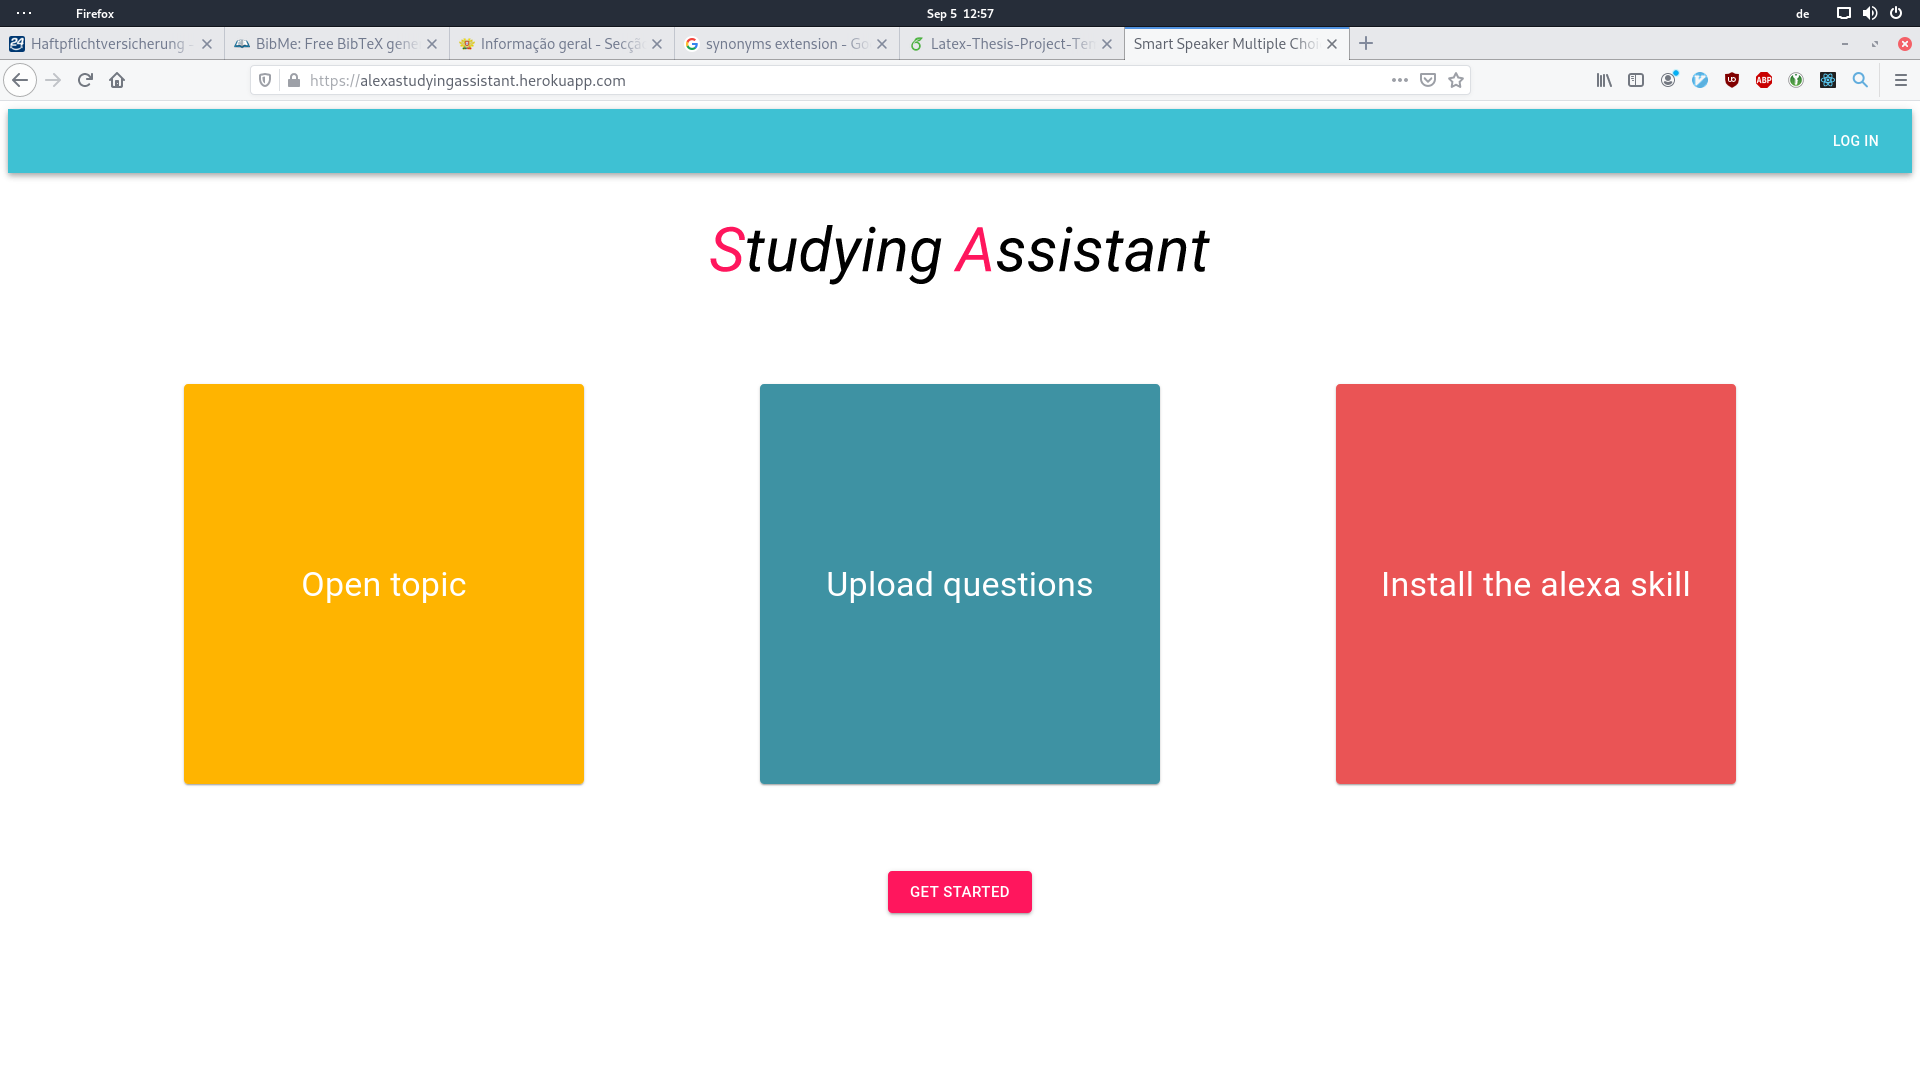
\includegraphics[width=.9\linewidth]{images/app/asa/homepage.png}
  \caption{Homepage of the web application.}
  \label{fig:homepage}
 \end{figure}
 
 \begin{figure}
  \centering
  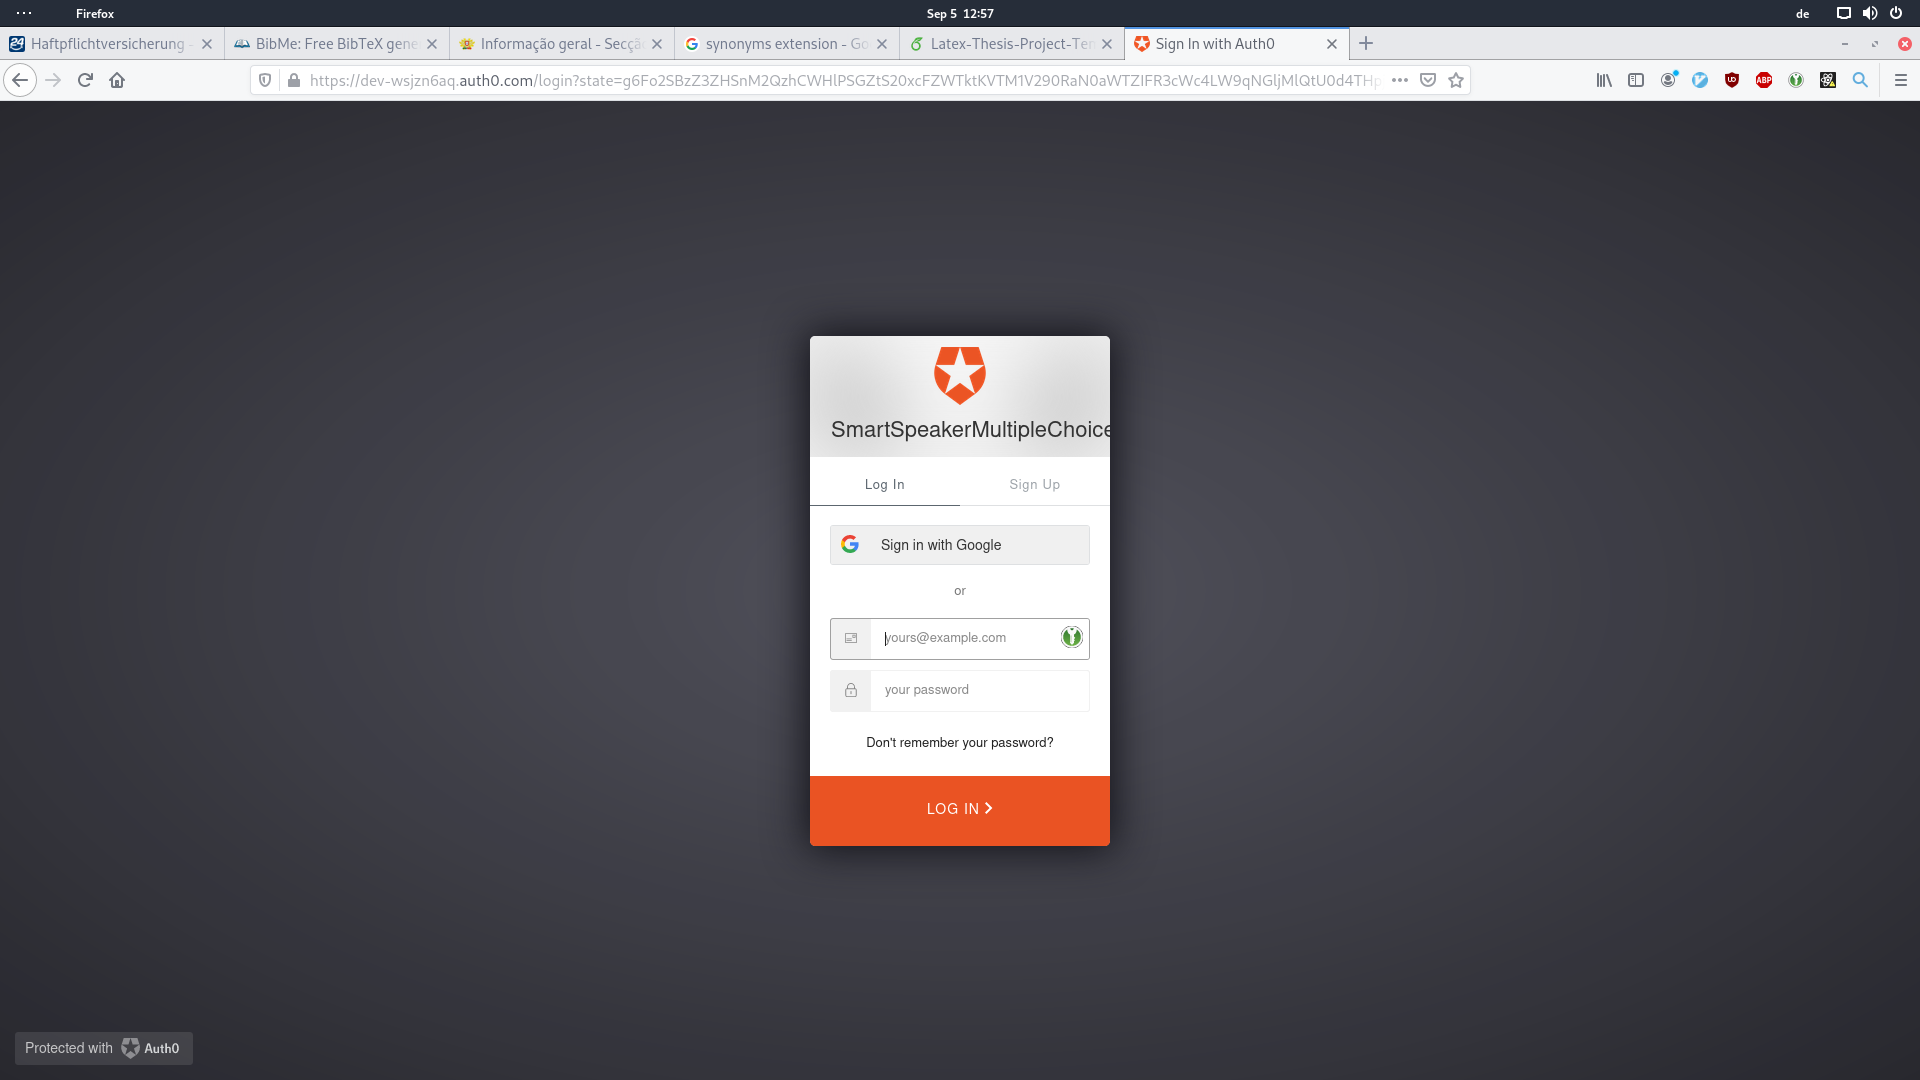
\includegraphics[width=.9\linewidth]{images/app/asa/auth0.png}
  \caption{Login dialog via Auth0 plugin.}
  \label{fig:login}
 \end{figure}


\subsection{Topic Creation}
After being logged in users can create 
or join topics in topic selection page. The user is prompted with a text field that 
uses fuzzy finding, as shown in \ref{fig:topic_search} to quickly narrow the search down to similar topics available.
If none was found, the user can press the Create button which opens a creation dialog \ref{fig:topic_creation}.

 \begin{figure}
  \centering
  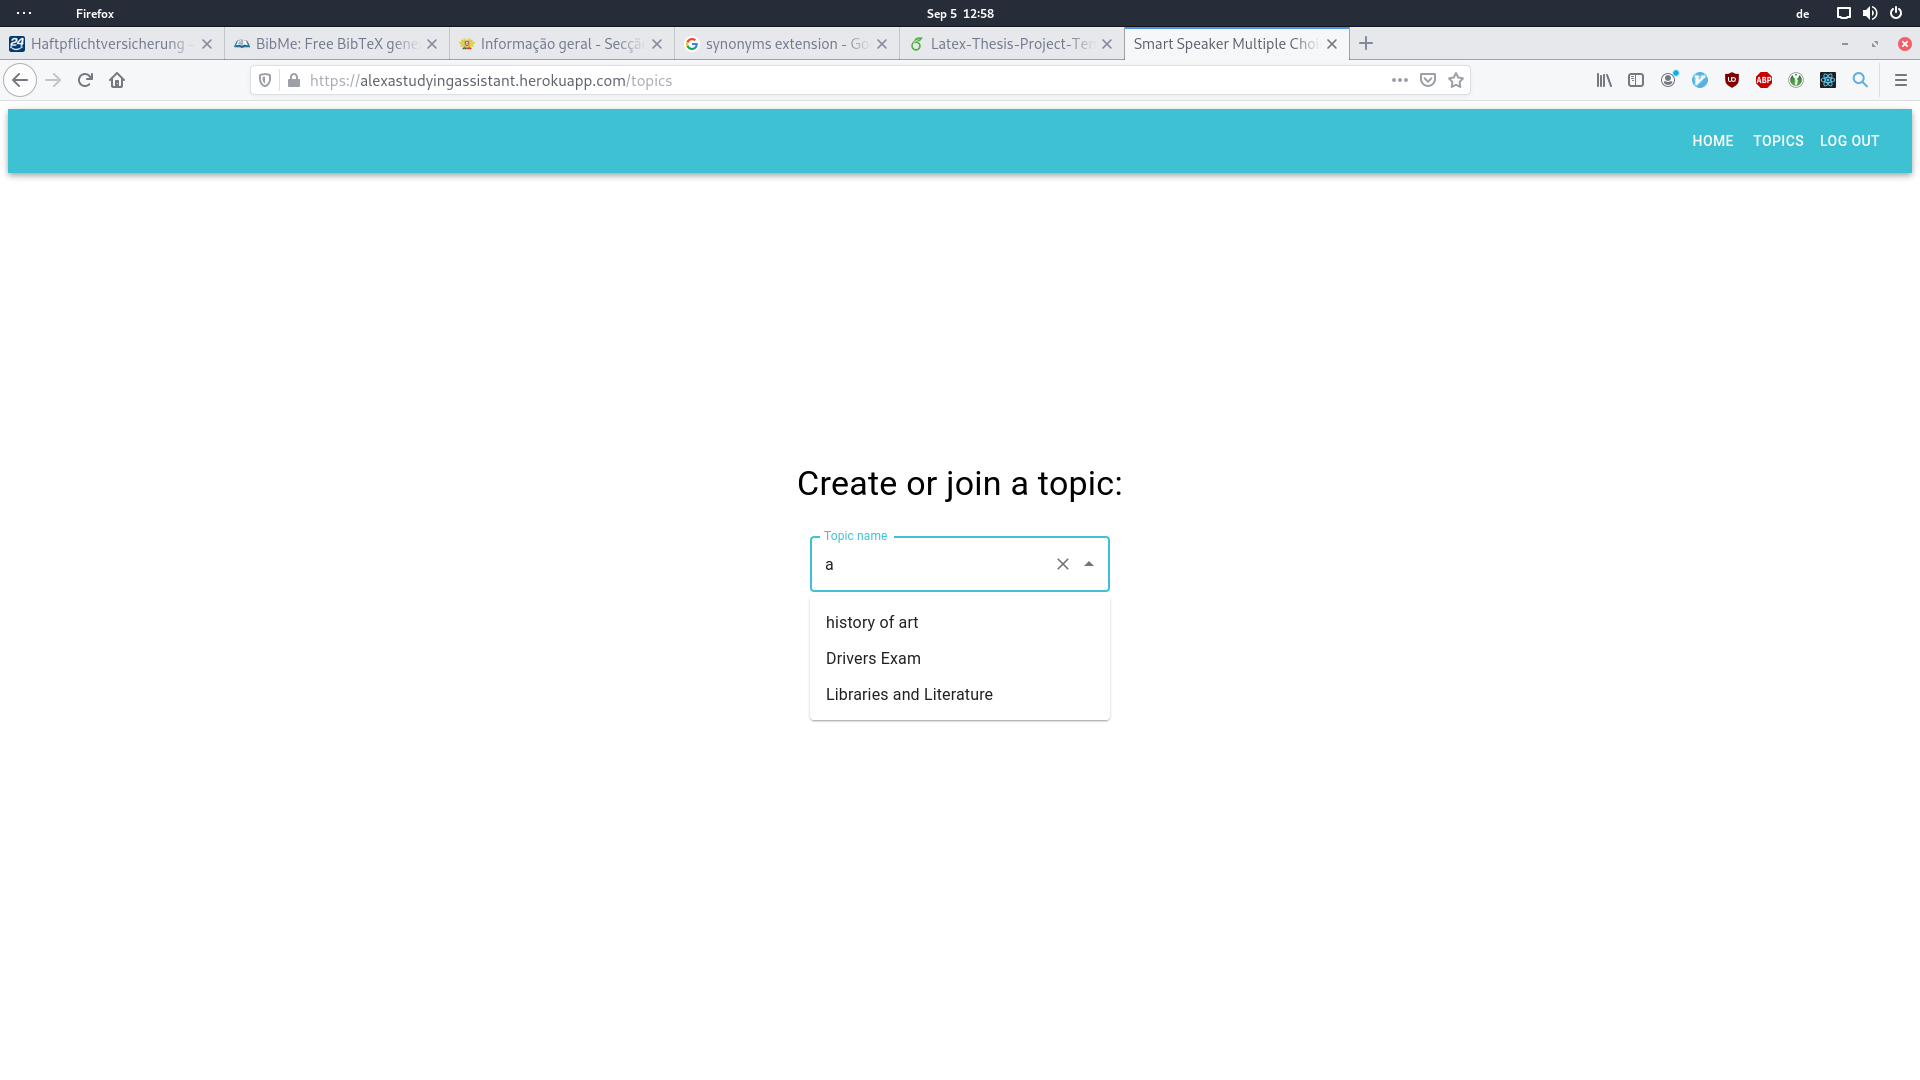
\includegraphics[width=.9\linewidth]{images/app/asa/topic_selection2.png}
  \caption{The search for the topics uses a fuzzy finding mechanism.}
  \label{fig:topic_search}
 \end{figure}
 
 \begin{figure}
  \centering
  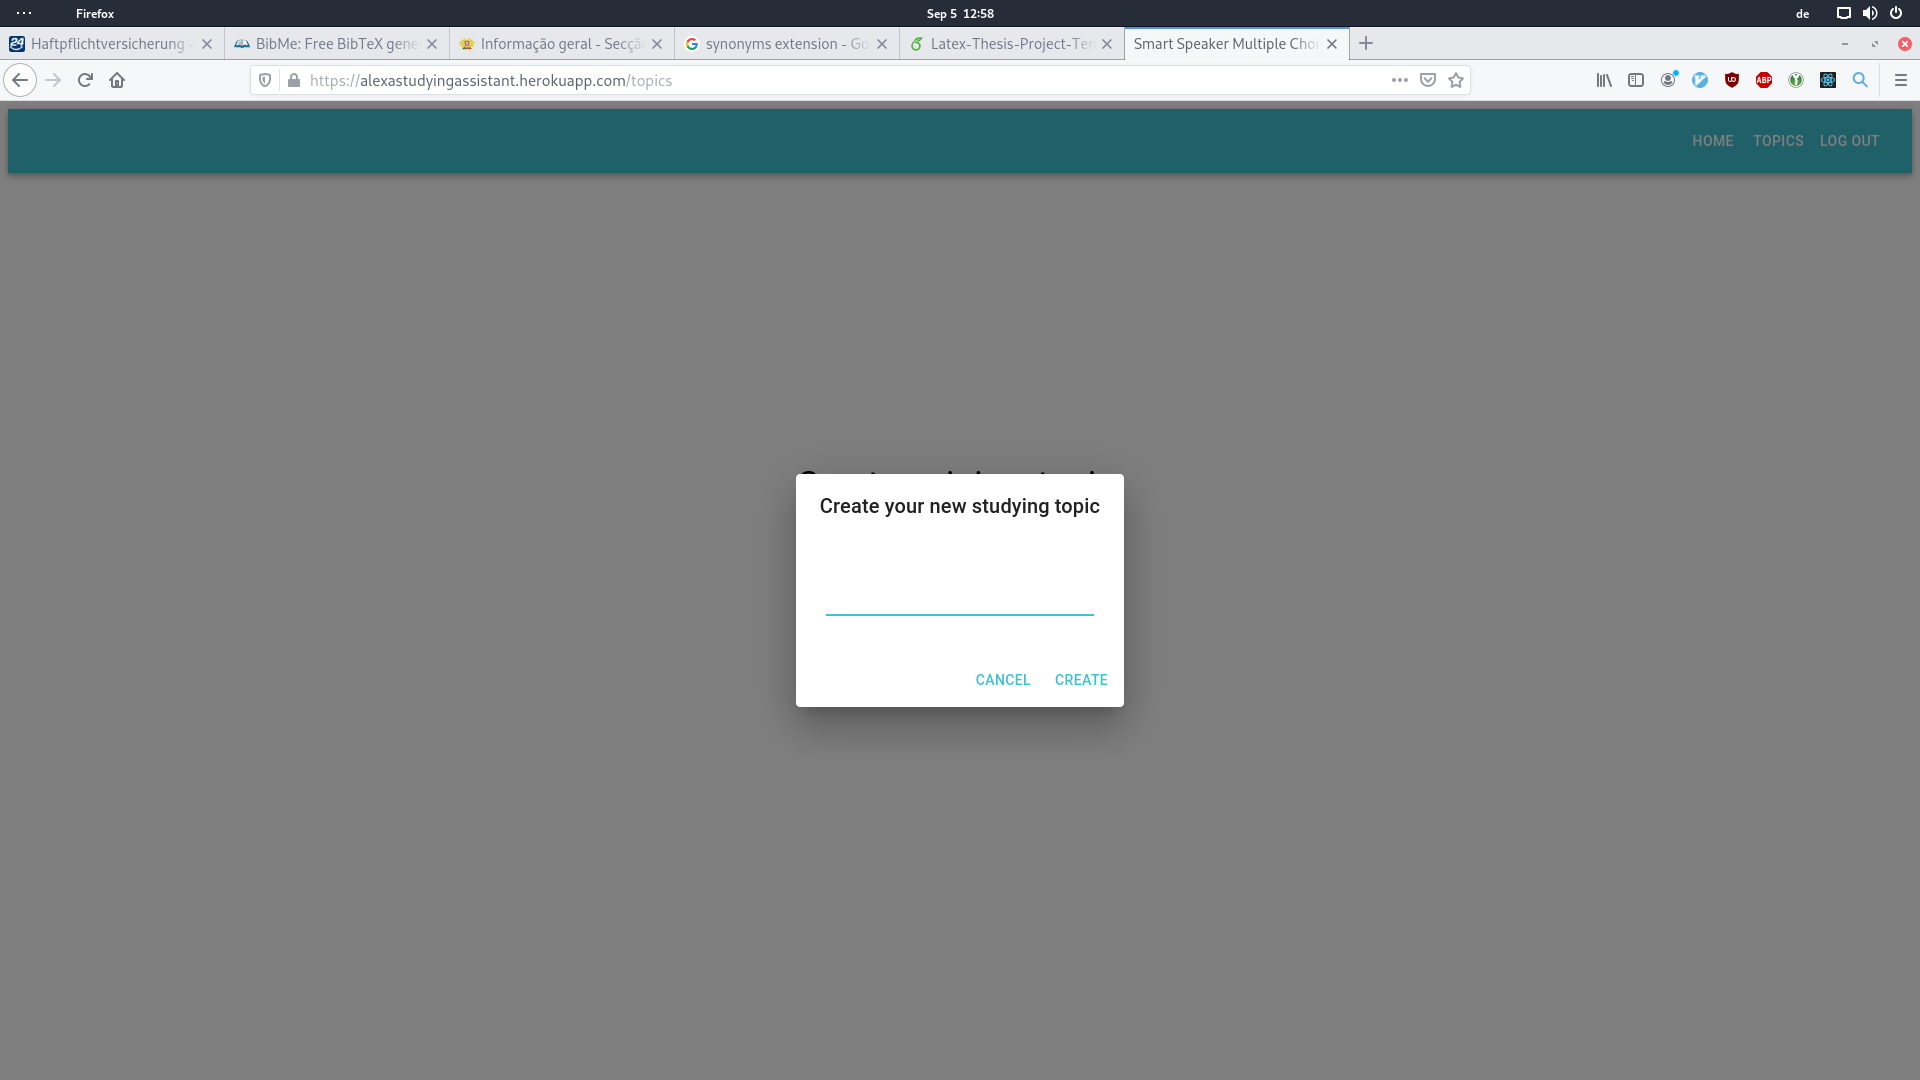
\includegraphics[width=.9\linewidth]{images/app/asa/topic_creation.png}
  \caption{An example of a topic creation.}
  \label{fig:topic_creation}
 \end{figure}

\subsection{Questions and Textbooks}
After they have created or loaded a topic they will have two columns, one showing a list with
all the textbooks provided by other users, the other with the list of all questions
currently associated with the given topic \ref{fig:topic}.

Both lists consist of expandable blocks which show firstly just the titles of both
questions and textbooks and on click expand to show everything, which is the entire
contents of the textbook on one hand and the multiple choice answers with the 
correct marked one on the other.

The idea behind this piece of software was to have commonly useful snippets of text
with valuable information begin available at the time of creation of the new questions,
so that for instance, if a user is currently studying in a course and wants to 
practice a given topic, he can upload the corresponding textbook, read paragraph by 
paragraph on the website and create questions as he comes up with important concepts
we wishes to study.

\begin{figure}
  \centering
  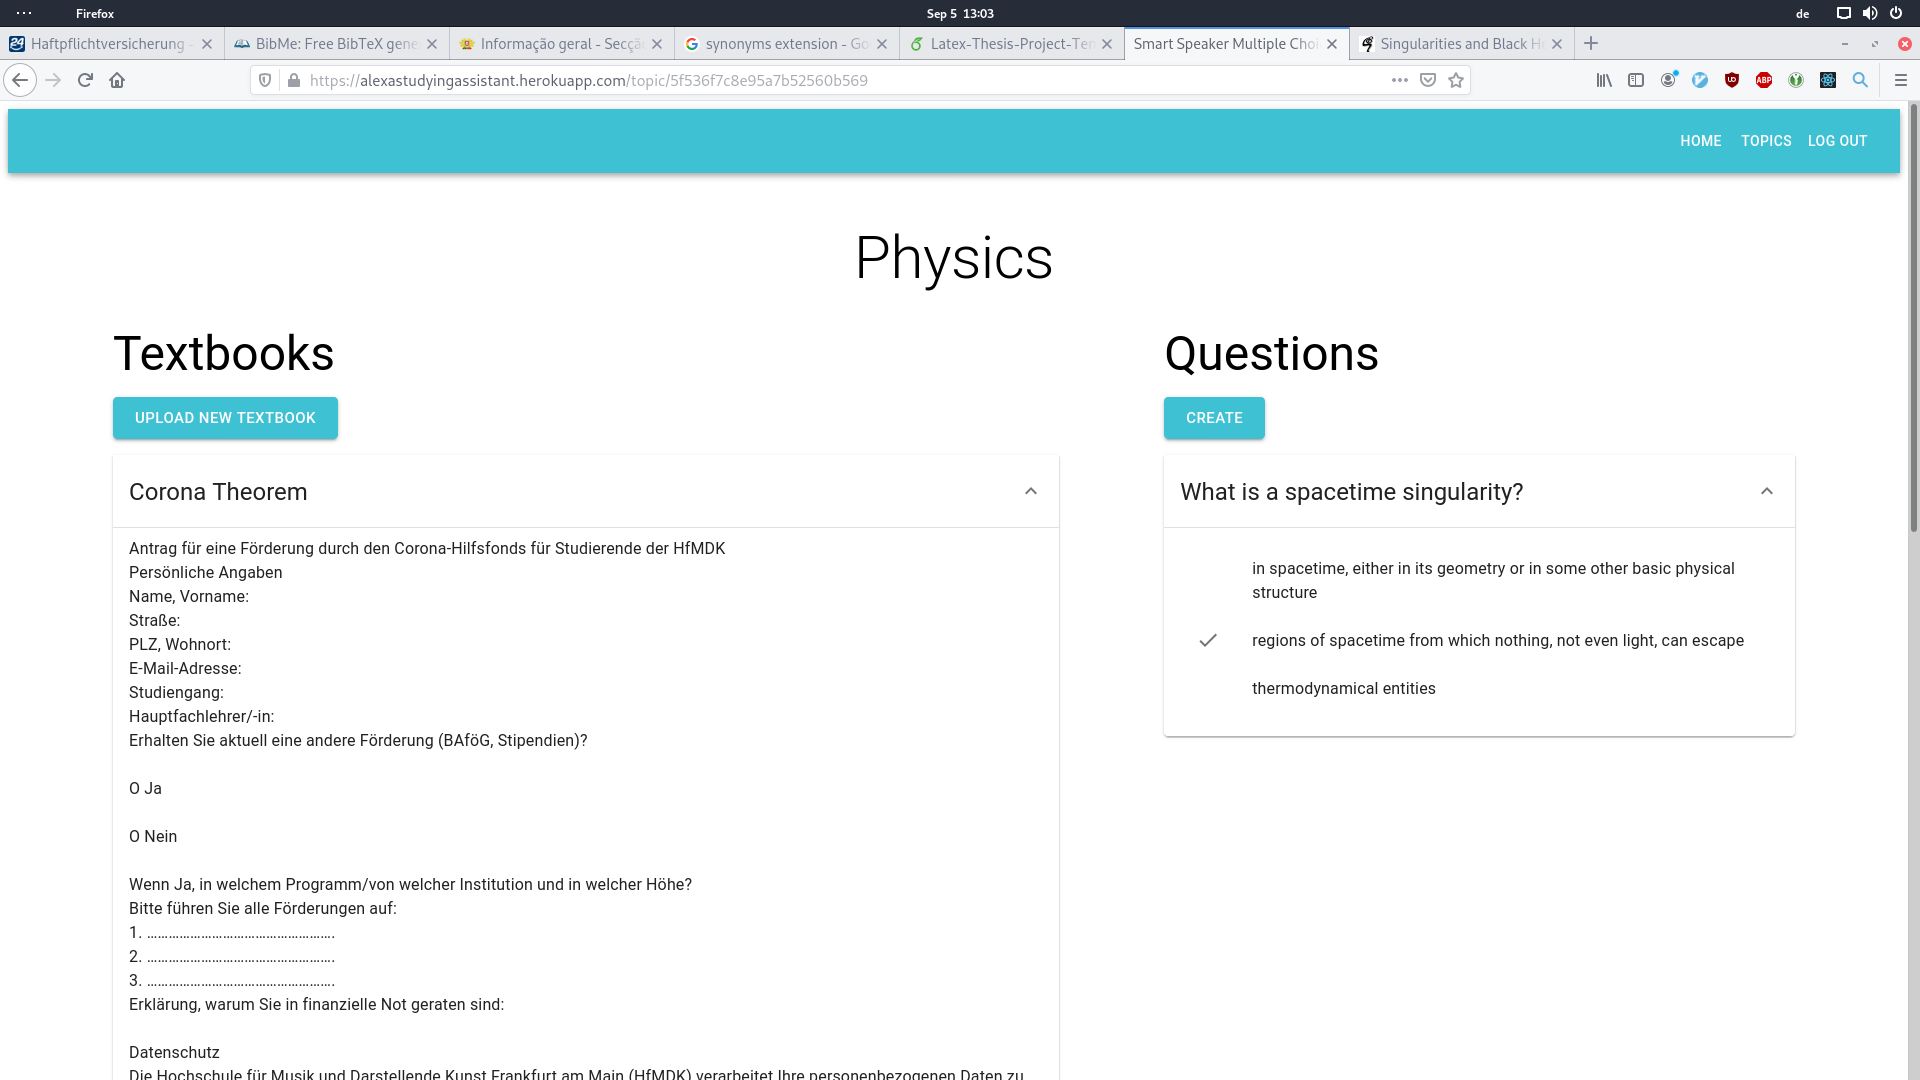
\includegraphics[width=.9\linewidth]{images/app/asa/topic.png}
  \caption{Two columns with the uploaded textbooks and questions for referencing and studying 
    inside the app.
  }
  \label{fig:topic}
\end{figure}
 
 
\subsection{Potential Future Improvements}
\label{subsection:future}
Another reason behind these parallel layout would be to easily add a feature in the future
where students could bind given questions to a given textbook, or even a given location
in the textbook, so that questions could be sorted by textbook or by chapter, etc.
Also a similar idea, would be to read text snippets from each textbook out load 
by the alexa skill, and prompt the related questions by the end of each paragraph for
example. All of the aforementioned ideas can be easily incorporated in the web application
by either creating new short components or by extending the existing ones.


\subsection{Upload Dialogs}

\begin{figure}
  \centering
  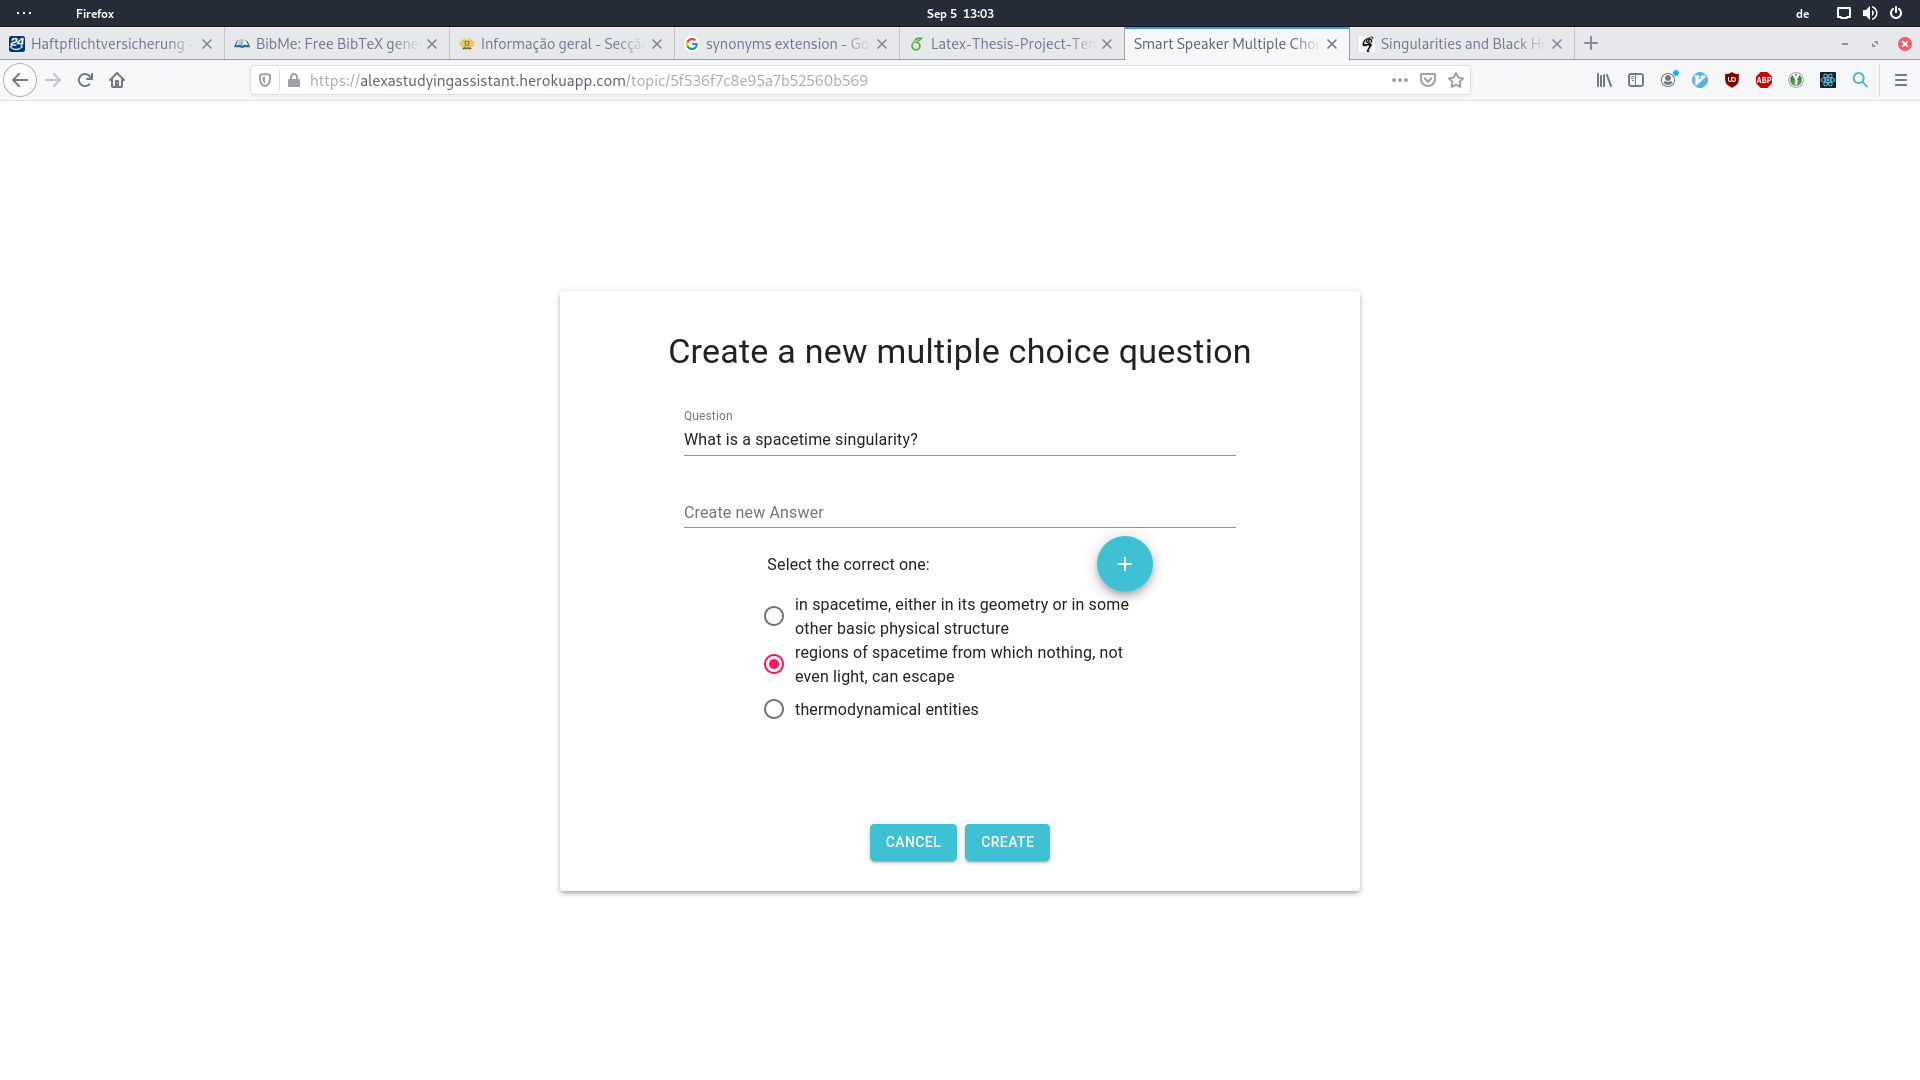
\includegraphics[width=.9\linewidth]{images/app/asa/question_creation.png}
  \caption{
    The upload dialog for questions. The user can add as many answers as he/she wishes and
    select the correct one.
  }
  \label{fig:questions}
\end{figure}

\begin{figure}
  \centering
  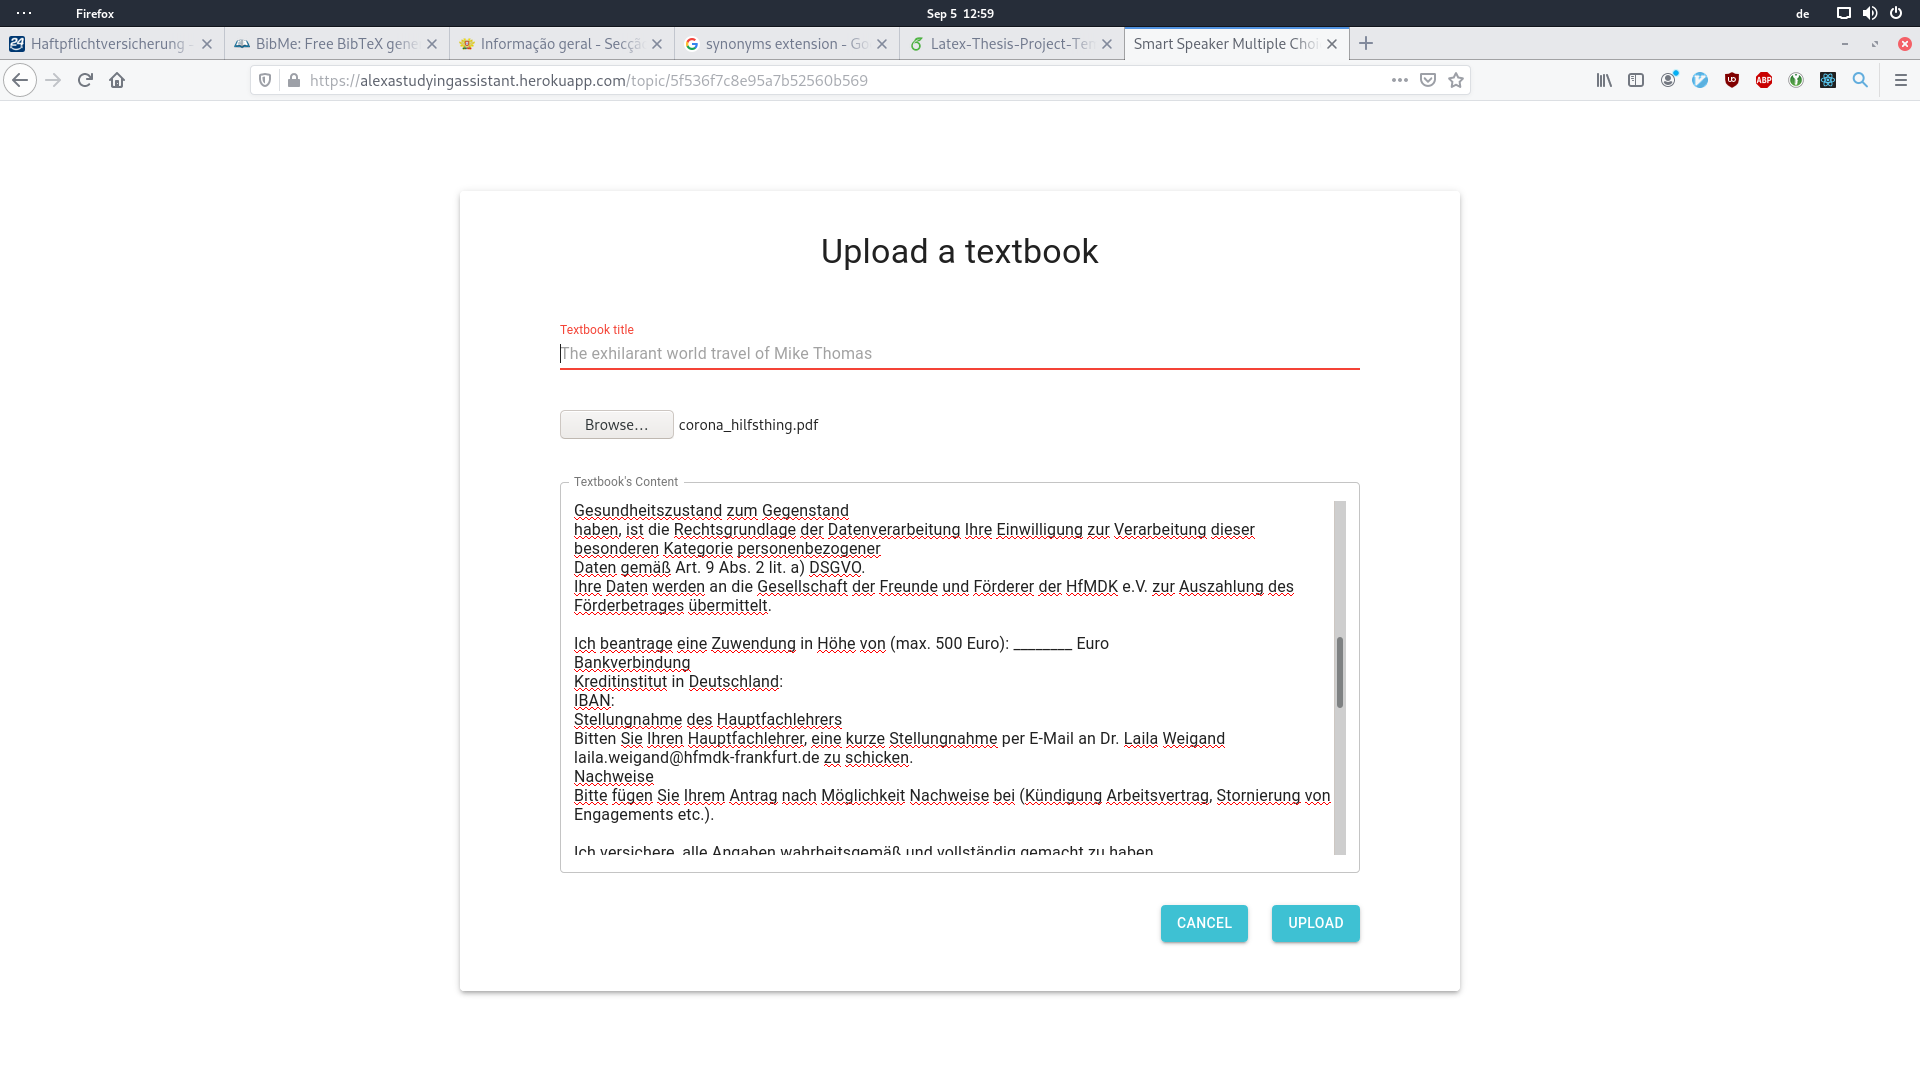
\includegraphics[width=.9\linewidth]{images/app/asa/textbook_upload.png}
  \caption{
    The upload dialog for textbooks. It can convert a large pdf file to text which can be
    marked and manipulated more easily.
  }
  \label{fig:textbooks}
\end{figure}

The following shows the Dialogs shown when a user wants to upload a textbook (\ref{fig:textbooks}) or question (\ref{fig:questions}).
For the textbook uploads, a functionality was written in the server side back-end of
the application, where one can upload the contents on the textbook and it will be 
translated from PDF format to plain text and added to the input field. This ability
has many advantages. Firstly, all text content is saved in the same format, and one
that's easily changeable. Second, its format that can be send via HTML and directly
read by the alexa skill. And third, it will be easier to add tags in the end of each 
sentence, paragraph, chapter, etc, by writing extra words in the middle of the text.

The question Dialog shows a very easy form with only two fields, and the user can add 
any variable number of answers for each question.

\section{User Management}

Another non visible, but important feature is that all uploads are assigned to a user ID, 
meaning that in the future following all the uploads and content from another user, or
even creating groups with common interests, hence creating a proper Community of Practice
would be trivial. All of these were left, since the idea was to just create the basic 
functionalities to interact with a smart speaker and assess if that functionality in itself
with be enough to attract and gather new users for newer niche technologies with the
intend of learning.


\subsection{Additional Technologies}

Besides the main technologies used as a skeleton for the web application, 
the following additional tools are also essential:

\begin{itemize}
\item \textbf{Docker:} One of the most popular tools for DevOps of our times. Docker 
    containerization does two things. It makes deployment of the web application completely
    cross platform and it creates an important layer of security and sandboxing 
    via its containerization process.

\item \textbf{Heroku:} \textit{A cloud platform that lets companies build, deliver, monitor and 
    scale apps — we're the fastest way to go from idea to URL, bypassing all those 
    infrastructure headaches} \cite{heroku}. Meaning, the perfect setup to quickly deploy a docker
    container with the existing web application and to start testing with real users.
    Another big advantage of Heroku is that it uses certified SSL endpoints recognized
    by the Amazon Web Services, which means the alexa hosted skill can communicate 
    with a server deployed in Heroku without further configuration.

\end{itemize}

\section{Alexa Skill}

The Alexa Skill is the other half of the application and contains the essential
part of its interaction.
As the name of the thesis implies, the core and principle point of 
the project is to create an interactive learning experience using a smart speaker,
although in reality the creation and connection between users during the process
of creation topics and questions is just as important as the latter. Nonetheless
same features provided by the skill were key and essential to the whole experience.

As most smart speaker applications, there is a fine balance needed for its success.
The skill needs first and foremost to simplify the whole procedure of sitting down 
reading the multiple choice questions from either cards (which would consume a lot 
of time in their construction) or from the website or different sources, followed
by a straightforward conversation with the device, where users can practice 
simultaneously with other daily tasks, say washing the dishes, hanging clothes,
sweeping the floors or even just by laying down in the couch. Whether this habits
are effective or not is a whole different question and like with many things matters
studying in pedagogy, this will most likely depend on the student. The main point
that needs to be covered by the skill is to demonstrate the ability and 
practicality to study and interact with the smart speaker device in a much 
simpler and effortless way.

For this to be achieved, a compromise had to be found regarding how to dose the 
features provided by the skill and their clarity. It was settled to solely use 
the speaker to fetch all questions from the web server given a topic title posing
them to the user and keeping track of the correct answer pro question ratio.
Besides this basic usage the skill can also explain how to upload and create more
questions if needed. The pictures below show a valid conversation with the smart
speaker \ref{fig:start} \ref{fig:interaction} \ref{fig:change_topic} \ref{fig:stop}.


\begin{figure}[!tbp]
  \centering
  \begin{minipage}[b]{0.4\textwidth}
    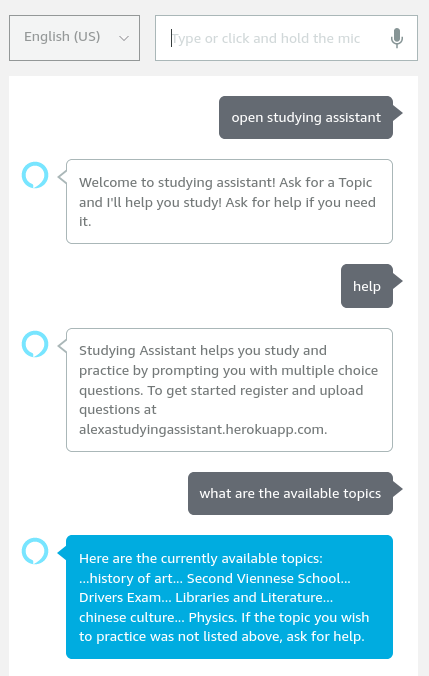
\includegraphics[width=\textwidth]{images/app/studying_assistant/start.png}
    \caption{Starting conversation with alexa skill.}
    \label{fig:start}
  \end{minipage}
  \hfill
  \begin{minipage}[b]{0.4\textwidth}
    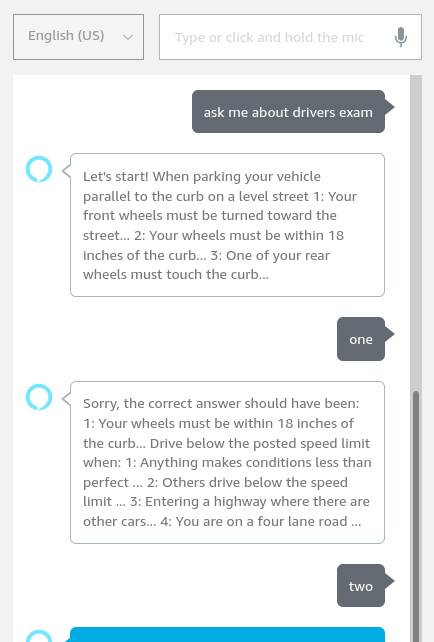
\includegraphics[width=\textwidth]{images/app/studying_assistant/interaction1.png}
    \caption{Example of interaction after request to study given topic.}
    \label{fig:interaction}
  \end{minipage}
\end{figure}

\begin{figure}[!tbp]
  \centering
  \begin{minipage}[b]{0.4\textwidth}
    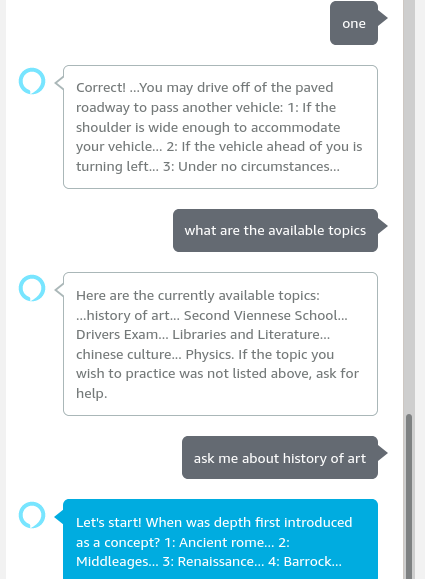
\includegraphics[width=\textwidth]{images/app/studying_assistant/change_topic.png}
    \caption{
        Example of the user asking the alexa skill to switch the topic to be studied.
    }
    \label{fig:change_topic}
  \end{minipage}
  \hfill
    \begin{minipage}[b]{0.4\textwidth}
    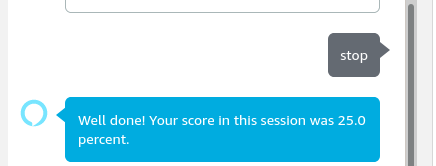
\includegraphics[width=\textwidth]{images/app/studying_assistant/stop.png}
    \caption{
        Alexa let's you know the session's score after closing the skill.
    }
    \label{fig:stop}
  \end{minipage}
\end{figure}



\subsection{User Management Roles}

The user management roles differ in the alexa skill from the web application.
This was a design choice which might change in the future if needed. While
the web application stores all public question, textbook and topic creation to
a given user or email with the OAuth protocol, the skill solely keeps track
of the sessions. The reason behind this decision, lies on the fact that 
users will very likely want to repeat the same multiple choice questions more 
than once to practice even if no new questions were uploaded. \textit{Repetitio 
est mater studiorum; Repetition is the mother of all learning.}

Accordingly once a user starts to interact with the smart speaker, a session is
loaded where it keeps track of all answered questions pro topic, so if the student
switches between topics and later returns, the last prompted question will still be prompted
and no question will be repeated. Additionally, every time a session starts a topic
is selected all its questions are shuffled so the user learns the proper answers
and not the correct order of answers.

\subsection{Python Hosted Skill}

Originally the Go Programming Language was selected to write the implementation 
of the alexa skill for the same reasons referred previously in its description.
This plan changed to the alternative Python Programming Language since the 
Amazon Web Services allow developers to host in a local server as an incentive, 
that greatly simplifies and secures any vulnerabilities in the communication
between skill and smart speaker device.

Another great advantage of having an alexa skill hosted by the AWS is the 
uncomplicated process of publishing the skill. This process is undertaking at the 
moment, and most of the third party certification was skipped.



\section{Application Workflow}

The whole workflow of the skill ends up being fairly straightforward, the user 
simply needs to:

\begin{enumerate}
        \item Visit the https://alexastudyingassistant.herokuapp.com.
        \item Join or create a topic to study.
        \item Upload questions or textbooks to share with other users.
        \item Download and install the alexa skill \textbf{Studying Assistant}
        \item Start the interaction by launching the skill.
        \item Ask the available topics or start practice a given one.
        \item Stop when done and check for the score.
\end{enumerate}

This workflow is of course divided in two steps, but users could and should 
just iterate more often between the 5th and 7th step.


\section{Summary}

In a nutshell, in this chapter the basic architecture and potential of both
applications, both the alexa skill and the web server and website were described.
Some suggestions were also made on ways how the software could grow in the near 
future, and although all the source code was unrevealed, the latter can be examined
following the URL, 
\href{https://github.com/jmpargana/AlexaStudyingAssistant}{https://github.com/jmpargana/AlexaStudyingAssistant}, where a
public open-source licensed repository was published.